\documentclass[12pt]{beamer}
\usepackage{../Estilos/BeamerMAF}
\usepackage{../Estilos/ColoresLatex}
%Sección para el tema de beamer, con el theme, usercolortheme y sección de footers
\usetheme{Frankfurt}
\usecolortheme{beaver}
%\useoutertheme{default}
\setbeamercovered{invisible}
% or whatever (possibly just delete it)
\setbeamertemplate{section in toc}[sections numbered]
\setbeamertemplate{subsection in toc}[subsections numbered]
\setbeamertemplate{subsection in toc}{\leavevmode\leftskip=3.2em\rlap{\hskip-2em\inserttocsectionnumber.\inserttocsubsectionnumber}\inserttocsubsection\par}
% \setbeamercolor{section in toc}{fg=blue}
% \setbeamercolor{subsection in toc}{fg=blue}
% \setbeamercolor{frametitle}{fg=blue}
\setbeamertemplate{caption}[numbered]

\setbeamertemplate{footline}
\beamertemplatenavigationsymbolsempty
\setbeamertemplate{headline}{}


\makeatletter
% \setbeamercolor{section in foot}{bg=gray!30, fg=black!90!orange}
% \setbeamercolor{subsection in foot}{bg=blue!30!yellow, fg=red}
% \setbeamercolor{date in foot}{bg=black, fg=white}
\setbeamertemplate{footline}
{
  \leavevmode%
  \hbox{%
  \begin{beamercolorbox}[wd=.333333\paperwidth,ht=2.25ex,dp=1ex,center]{section in foot}%
    \usebeamerfont{section in foot} \insertsection
  \end{beamercolorbox}%
  \begin{beamercolorbox}[wd=.333333\paperwidth,ht=2.25ex,dp=1ex,center]{subsection in foot}%
    \usebeamerfont{subsection in foot}  \insertsubsection
  \end{beamercolorbox}%
  \begin{beamercolorbox}[wd=.333333\paperwidth,ht=2.25ex,dp=1ex,right]{date in head/foot}%
    \usebeamerfont{date in head/foot} \insertshortdate{} \hspace*{2em}
    \insertframenumber{} / \inserttotalframenumber \hspace*{2ex} 
  \end{beamercolorbox}}%
  \vskip0pt%
}







\setbeamercolor{section in foot}{bg=deepcarmine, fg=white}
\setbeamercolor{subsection in foot}{bg=flame, fg=white}
\setbeamercolor{date in foot}{bg=blue, fg=white}

\makeatletter
\setbeamertemplate{footline}
{
\leavevmode%
\hbox{%
\begin{beamercolorbox}[wd=.333333\paperwidth,ht=2.25ex,dp=1ex,center]{section in foot}%
  \usebeamerfont{section in foot} \insertsection
\end{beamercolorbox}%
\begin{beamercolorbox}[wd=.333333\paperwidth,ht=2.25ex,dp=1ex,center]{subsection in foot}%
  \usebeamerfont{subsection in foot}  \insertsubsection
\end{beamercolorbox}%
\begin{beamercolorbox}[wd=.333333\paperwidth,ht=2.25ex,dp=1ex,right]{date in head/foot}%
  \usebeamerfont{date in head/foot} \insertshortdate{} \hspace*{1.5em}
  \insertframenumber{} / \inserttotalframenumber \hspace*{2ex} 
\end{beamercolorbox}}%
\vskip0pt%
}
\makeatother
\usefonttheme{serif}
\setbeamercolor{frametitle}{bg=lavenderblue}
\resetcounteronoverlays{saveenumi}

\date{26 de abril de 2022}

\title{\large{La parte angular del átomo de hidrógeno}}
\subtitle{Funciones Especiales I}
\author{M. en C. Gustavo Contreras Mayén}

\begin{document}
\maketitle
\fontsize{14}{14}\selectfont
\spanishdecimal{.}

\section*{Contenido}
\frame[allowframebreaks]{\tableofcontents[currentsection, hideallsubsections]}

%Ref. El átomo de hidrógeno
\section{La función de onda}
\frame{\tableofcontents[currentsection, hideothersubsections]}
\subsection{Ecuación separable}

\begin{frame}
\frametitle{La función de onda}
De la revisión del problema del átomo de hidrógeno, mediante la técnica de separación de variables, es posible deducir la expresión de la función de onda:
\pause
\begin{align}
\psi_{n, \ell, m} (r, \theta, \phi) = R _{n, \ell} (r) \, \Theta_{\ell, m} (\theta) \, \Phi_{m} (\phi)
\label{ec:ecuacion_07_25}
\end{align}
\end{frame}
\begin{frame}
\frametitle{Condiciones para la función}
Tendremos esta función de onda para cada terna de números cuánticos que satisfagan las condiciones:
\pause
\begin{eqnarray}
\begin{aligned}
n &\geq 1 \hspace{0.2cm} n = 1, 2, 3, \ldots \\[0.5em] \pause
\ell &= 0, 1, \ldots, (n - 1) \\[0.5em] \pause
m &= \ell, \ell - 1, \ldots, 0, - \ell + 1, -\ell
\end{aligned}
\label{eq:ecuacion_07_26}
\end{eqnarray}
pues en otro caso, no es posible satisfacer las condiciones de frontera. \pause Las funciones de onda del hidrógeno, reciben también el nombre de \emph{orbitales atómicos}.
\end{frame}
\begin{frame}
\frametitle{Revisando las funciones}
Por ejemplo, con $n = 2$ \pause veremos cuántas funciones de onda pueden construirse:
\pause
\setbeamercolor{item projected}{bg=ballblue,fg=white}
\setbeamertemplate{enumerate items}{%
\usebeamercolor[bg]{item projected}%
\raisebox{1.5pt}{\colorbox{bg}{\color{fg}\footnotesize\insertenumlabel}}%
}
\begin{enumerate}[<+->]
\item $\ell$ solo puede tomar los valores $\ell = 0, 1$.
\item En el primer caso $m$ solo puede valer $m = 0$.
\item Mientras que para $\ell = 1$, $m = -1, 0, 1$.
\end{enumerate}
\end{frame}
\begin{frame}
\frametitle{Cuatro funciones obtenidas}
Es decir, se pueden obtener cuatro funciones de onda:
\pause
\begin{eqnarray*}
\begin{aligned}
\psi_{2, 0, 0} (r, \theta, \phi) &= R_{2, 0} (r) \, \Theta_{0, 0} (\theta) \, \Phi_{0} (\phi) \\[0.5em] \pause
\psi_{2, 1, 1} (r, \theta, \phi) &= R_{2, 1} (r) \, \Theta_{1, 1} (\theta) \, \Phi_{1} (\phi)
\end{aligned}
\end{eqnarray*}
\end{frame}
\begin{frame}
\frametitle{Cuatro funciones obtenidas}
\begin{eqnarray*}
\begin{aligned}
\psi_{2, 1, 0} (r, \theta, \phi) &= R_{2, 1} (r) \, \Theta_{1, 0} (\theta) \, \Phi_{0} (\phi) \\[0.5em] \pause
\psi_{2, 1, -1} (r, \theta, \phi) &= R_{2, 1} (r) \, \Theta_{1, -1} (\theta) \, \Phi_{-1} (\phi)
\end{aligned}
\end{eqnarray*}
Encontramos que la función radial de la primera es distinta a las otras tres, que tienen la misma descripción radial.
\end{frame}
\begin{frame}
\frametitle{¿Cómo son las funciones?}
Podríamos preguntarnos ahora: ¿qué forma adquiere la función radial $R_{2, 1} (r)$ \pause o la función angular $\Theta_{0, 0} (\theta) \, \Phi_{0} (\phi)$ del ejemplo anterior? 
\\
\bigskip
\pause
La respuesta es fácil de dar, lo difícil, es obtenerlas.
\end{frame}
\begin{frame}
\frametitle{Funciones radiales}
A continuación, presentaremos algunas funciones radiales  y angulares para el átomo de hidrógeno (tomaremos prestados los resultados), encontraremos que se incluyen funciones trigonométricas y exponenciales.
\end{frame}
\begin{frame}
\frametitle{El radio de Bohr}
El valor de $\pderivada{a}_{0}$ es el radio de Bohr calculado con la masa reducida $\mu$, es decir:
\pause
\begin{align}
\pderivada{a}_{0} = \dfrac{\hbar^{2}}{\kappa \, \mu \, e^{2}} = a_{0} \, \dfrac{m_{e}}{\mu}
\label{eq:ecuacion_07_27}
\end{align}
\end{frame}

\subsection*{Funciones radiales}

\begin{frame}
\frametitle{Funciones radiales}
\begin{table}[H]
\centering
\large
\renewcommand{\arraystretch}{1.5}
\begin{tabular}{|c | c | c|} \hline
$n$ & $\ell$ & $R_{n, \ell} (r)$ \\ \hline
$1$ & $0$ & $2 \bigg( \dfrac{Z}{\pderivada{a}_{0}} \bigg)^{\frac{3}{2}} \, \exp\bigg( \dfrac{Z r}{2 \pderivada{a}_{0}} \bigg)$ \\ \hline
$2$ & $0$ & $\dfrac{1}{2 \sqrt{2}} \bigg( \dfrac{Z}{\pderivada{a}_{0}} \bigg)^{\frac{3}{2}} \, \bigg( 2 - \dfrac{Z r}{\pderivada{a}_{0}} \bigg) \, \exp\bigg( \dfrac{Z r}{2 \pderivada{a}_{0}} \bigg)$ \\ \hline
$2$ & $1$ & $\dfrac{1}{2 \sqrt{6}} \bigg( \dfrac{Z}{\pderivada{a}_{0}} \bigg)^{\frac{3}{2}} \, \bigg( \dfrac{Z r}{\pderivada{a}_{0}} \bigg) \, \exp\bigg( \dfrac{Z r}{2 \pderivada{a}_{0}} \bigg)$ \\ \hline
\end{tabular}
%\caption{Funciones radiales del hidrógeno.}
%\label{table:Tabla_funciones_radiales}
\end{table}
\end{frame}
\begin{frame}
\frametitle{Funciones radiales}
\begin{table}[H]
\centering
\renewcommand{\arraystretch}{1.5}
\fontsize{12}{12}\selectfont
\begin{tabular}{|c | c | c|} \hline
$n$ & $\ell$ & $R_{n, \ell} (r)$ \\ \hline
$3$ & $0$ & $\dfrac{2}{81 \sqrt{3}} \bigg( \dfrac{Z}{\pderivada{a}_{0}} \bigg)^{\frac{3}{2}} \, \bigg[ 2 \bigg( \dfrac{Z r}{\pderivada{a}_{0}} \bigg)^{2} - 18 \bigg( \dfrac{Z r}{\pderivada{a}_{0}} \bigg) + 27 \bigg] \, \exp\bigg( \dfrac{Z r}{3\pderivada{a}_{0}} \bigg)$ \\ \hline
$3$ & $1$ & $\dfrac{2 \sqrt{2}}{81 \sqrt{3}} \bigg( \dfrac{Z}{\pderivada{a}_{0}} \bigg)^{\frac{3}{2}} \, \bigg[ 6 - 18 \bigg( \dfrac{Z r}{\pderivada{a}_{0}} \bigg) \bigg] \, \exp\bigg( \dfrac{Z r}{3\pderivada{a}_{0}} \bigg)$ \\ \hline
\end{tabular}
%\caption{Funciones radiales del hidrógeno.}
%\label{table:Tabla_funciones_radiales}
\end{table}
\end{frame}

\subsection*{Funciones angulares}

\begin{frame}
\frametitle{Funciones angulares}
\begin{table}[H]
\centering
\renewcommand{\arraystretch}{1.5}
\begin{tabular}{|c | c | c|} \hline
$\ell$ & $m$ & $\Theta_{\ell, m} (\theta) \, \Phi_{m} (\phi)$ \\ \hline
$0$ & $0$ & $(1/4 \pi)^{\frac{1}{2}}$ \\ \hline
$1$ & $0$ & $(3/4 \pi)^{\frac{1}{2}} \, \cos \theta$ \\ \hline
$1$ & $1$ & $(3/8 \pi)^{\frac{1}{2}} \, \sin \theta e^{i \phi}$ \\ \hline
$1$ & $-1$ & $(3/8 \pi)^{\frac{1}{2}} \, \sin \theta e^{-i \phi}$ \\ \hline
\end{tabular}
%\caption{Funciones angulares del hidrógeno.}
%\label{table:Tabla_funciones_angulares}
\end{table}
\end{frame}
\begin{frame}
\frametitle{Funciones angulares}
\begin{table}[H]
\centering
\renewcommand{\arraystretch}{1.5}
\begin{tabular}{|c | c | c|} \hline
$\ell$ & $m$ & $\Theta_{\ell, m} (\theta) \, \Phi_{m} (\phi)$ \\ \hline    
$2$ & $0$ & $(5/16 \pi)^{\frac{1}{2}} \, (3 \, \cos \theta - 1)$ \\ \hline
$2$ & $1$ & $(15/8 \pi)^{\frac{1}{2}} \, \sin \theta \, \cos \theta \, e^{i \phi}$ \\ \hline
$2$ & $-1$ & $(15/8 \pi)^{\frac{1}{2}} \, \sin \theta \, \cos \theta \, e^{-i \phi}$ \\ \hline
\end{tabular}
%\caption{Funciones angulares del hidrógeno.}
%\label{table:Tabla_funciones_angulares}
\end{table}
\end{frame}

\subsection{Notación}

\begin{frame}
\frametitle{Notación conveniente}
Se muestra a continuación la notación simbólica que se acostumbra utilizar para denotar a las funciones de onda.
\\
\bigskip
\pause
Cada una está caracterizada por los números $n, \ell$ y $m$.
\end{frame}
\begin{frame}
\frametitle{Notación con valores de $\ell$}
Es es usual la notación con los valores de $\ell$:
\pause
\begin{table}
\centering
\begin{tabular}{|c | c | l|} \hline
$\ell$ & Símbolo & Significado \\ \hline
$0$ & \emph{s} & Sharp (exacta) \\ \hline
$1$ & \emph{p} & Principal (principal) \\ \hline
$2$ & \emph{d} & Difuse (difusa) \\ \hline
\end{tabular}
%\caption{Símbolos para los valores de $\ell$.}
\label{table:Tabla_valores_l}
\end{table}
\end{frame}
\begin{frame}
\frametitle{Notación con valores de $\ell$}
\begin{table}
\centering
\begin{tabular}{|c | c | l|} \hline
$\ell$ & Símbolo & Significado \\ \hline    
$3$ & \emph{f} & Fundamental (fundamental) \\ \hline
$4$ & \emph{g} & Ninguno \\ \hline
$5$ & \emph{h} & Ninguno \\ \hline
\vdots & \vdots & \vdots \\ \hline    
\end{tabular}
%\caption{Símbolos para los valores de $\ell$.}
%\label{table:Tabla_valores_l}
\end{table}
\end{frame}
\begin{frame}
\frametitle{Ejemplo del uso de la notación}
Cuando se hace referencia a la función $2 p_{1}$:, es aquella con:
\setbeamercolor{item projected}{bg=ballblue,fg=white}
\setbeamertemplate{enumerate items}{%
\usebeamercolor[bg]{item projected}%
\raisebox{1.5pt}{\colorbox{bg}{\color{fg}\footnotesize\insertenumlabel}}%
}
\begin{enumerate}[<+->]
\item $n = 2$.
\item $\ell = 1$ .
\item $m = 1$.
\end{enumerate}
\end{frame}
\begin{frame}
\frametitle{Ejemplo del uso de la notación}
cuando se tiene la $3 d_{-2}$, se está definiendo a la función con:
\setbeamercolor{item projected}{bg=ballblue,fg=white}
\setbeamertemplate{enumerate items}{%
\usebeamercolor[bg]{item projected}%
\raisebox{1.5pt}{\colorbox{bg}{\color{fg}\footnotesize\insertenumlabel}}%
}
\begin{enumerate}[<+->]
\item $n = 3$.
\item $\ell = 2$ .
\item $m = -2$.
\end{enumerate}
\end{frame}
\begin{frame}
\frametitle{El caso de los orbitales}
En el caso de los orbitales $s$, donde $\ell = 0$ y $m$ no tiene otro posible valor más que cero, \pause se evita el subíndice que especifica $m$. 
\\
\bigskip
\pause
Por lo que, el orbital $4s$ será aquel con $n = 4$, $\ell = 0$ y $m = 0$.
\end{frame}

\section{Análisis de la parte angular}
\frame{\tableofcontents[currentsection, hideothersubsections]}
\subsection{Información de la función}

\begin{frame}
\frametitle{Información de la función de onda}
Es de mucho interés extraer toda la información posible de la función de onda del átomo de hidrógeno.
\\
\bigskip
\pause
Entre otras cosas, se puede analizar la \textcolor{burgundy}{densidad de la probabilidad} para el electrón y los valores precisos o promedio de otras variables, como la \textcolor{byzantium}{distancia al núcleo}, el \textcolor{candyapplered}{momento angular}, la \textcolor{chestnut}{energía cinética}, etc.
\end{frame}
\begin{frame}
\frametitle{Uso de la función de onda}
Consideremos el cuadrado de la función de onda, por lo que la densidad de probabilidad $\rho (r, \theta, \phi)$ es:
\pause
\begin{eqnarray}
\begin{aligned}[b]
\rho (r, \theta, \phi) &= \abs{\psi_{n, \ell, m} (r, \theta, \phi)}^{2} = \\[0.5em]
&= R_{n,\ell}^{2} (r) \, \Theta_{\ell,m}^{2} (\theta) \abs{\Phi_{m} (\phi)}^{2}
\end{aligned}
\label{eq:ecuacion_07_42}
\end{eqnarray}
Se revisará inicialmente la parte angular, es decir: $\Theta_{\ell,m}^{2} (\theta) \abs{\Phi_{m} (\phi)}^{2}$.
\end{frame}
\begin{frame}
\frametitle{La parte angular}
A la función:
\pause
\begin{align}
Y_{\ell, m} = \Theta_{\ell,m} (\theta) \,\Phi_{m} (\phi)
\label{eq:ecuacion_07_76}
\end{align}
Le llamaremos \textbf{\textcolor{cinnabar}{armónico esférico}}.
\end{frame}
\begin{frame}
\frametitle{Componente compleja}
La componente $\phi$ de los armónicos esféricos es una función compleja, \pause ya que como se revisa en la Tabla de funciones angulares, contiene factores del tipo $e^{i m \phi}$. 
\end{frame}
\begin{frame}
\frametitle{Manejo de funciones reales}
Sin embargo, se puede demostrar cómo con una combinación adecuada de los armónicos esféricos, se producen solamente funciones de valor real, conocidas como \textbf{\textcolor{coolblack}{armónicos esféricos reales}}.
\end{frame}

\subsection{Armónicos esféricos reales}

\begin{frame}
\frametitle{Gráfica de los orbitales}
Si queremos graficar en coordenadas polares las partes angulares de los orbitales del hidrógeno, \pause se presenta un grave problema: la función $\Phi_{m} (\phi) = (1/2 \pi)^{\frac{1}{2}} \, e^{i m \phi}$ toma valores complejos.
\end{frame}
\begin{frame}
\frametitle{Caso especial}
Mientras $m = 0$, no hay problema alguno, \pause pero si el valor no es cero, no queda claro cómo graficar sobre la coordenada $r$ una distancia compleja.
\end{frame}
\begin{frame}
\frametitle{Uso de una identidad}
Las partes real e imaginaria de estas funciones, se recuperan con la identidad de Euler:
\pause
\begin{align}
e^{i m \phi} = \cos m \phi + i \, \sin m \phi
\label{eq:ecuacion_07_79}
\end{align}
\end{frame}
\begin{frame}
\frametitle{Uso del módulo}
Una manera de evitar los números complejos es trabajar con el módulo de los mismos, que es un número real.
\\
\bigskip
\pause
Por lo tanto, el módulo de la ec. (\ref{eq:ecuacion_07_79}), es:
\pause
\begin{align}
\abs{e^{i m \phi}} = \sqrt{ \cos^{2} m \phi + \sin^{2} m \phi} = 1
\label{eq:ecuacion_07_80}
\end{align}
\end{frame}
\begin{frame}
\frametitle{Funciones con $m \neq 0$}
Las primeras funciones donde aparece $m \neq 0$ \pause son la $p_{+1}$ y la $p_{-1}$ que, al revisar los valores de la Tabla de funciones angulares, son:
\pause
\begin{eqnarray}
\begin{aligned}
Y_{1, 1} (\theta, \phi) &= \bigg( \dfrac{3}{8} \bigg)^{\frac{1}{2}} \, \sin \theta \, e^{i \phi} \label{eq:ecuacion_07_81} \\[0.5em]
Y_{1, -1} (\theta, \phi) &= \bigg( \dfrac{3}{8} \bigg)^{\frac{1}{2}} \, \sin \theta \, e^{-i \phi} 
\end{aligned}
\label{eq:ecuacion_07_82}
\end{eqnarray}
\end{frame}
\begin{frame}
\frametitle{Calculando el módulo}
Ocupando la ec. (\ref{eq:ecuacion_07_80}), el módulo de ambas funciones es idéntico:
\pause
\begin{align}
\abs{Y_{1, 1} (\theta, \phi)} = \abs{Y_{1, -1} (\theta, \phi)} = \bigg( \dfrac{3}{8} \bigg)^{\frac{1}{2}} \, \sin \theta
\label{eq:ecuacion_07_83}
\end{align}
\end{frame}
\begin{frame}
\frametitle{Gráfica de la función}
Un esbozo de la gráfica de esta función en coordenadas polares se muestra en la figura:
\pause
\begin{figure}[H]
    \centering
    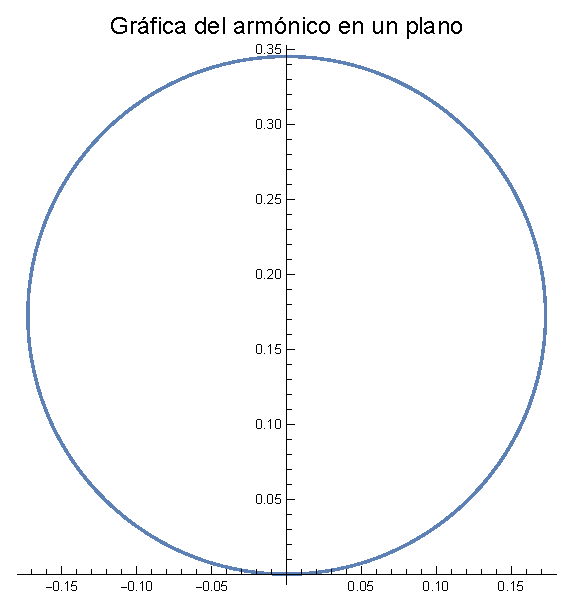
\includegraphics[scale=0.48]{Imagenes/Plot_Y11_01.eps}
    \caption{Gráfica del $\abs{Y_{1, 1} (\theta, \phi)}$ en el plano.}
    %\label{fig:figura_plot_Y11_01}
\end{figure}
\end{frame}
\begin{frame}
\frametitle{Gráfica en el  espacio}
En la siguiente figura se presenta la misma función, pero ahora al graficarla en el espacio:
\pause
\begin{figure}[H]
    \centering
    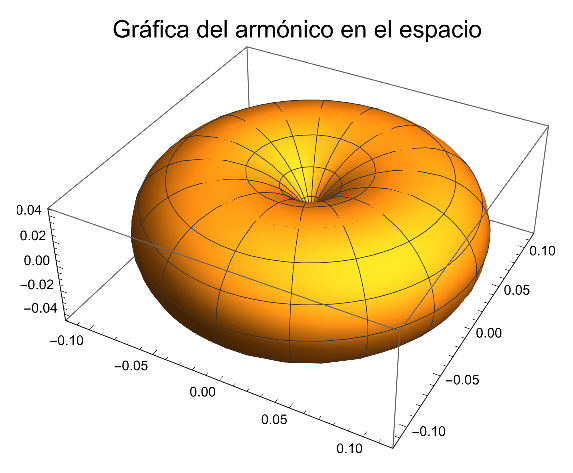
\includegraphics[scale=0.7]{Imagenes/Plot_Y11_02.eps}
    %\caption{Gráfica del $\abs{Y_{1, 1} (\theta, \phi)}$ en el espacio.}
    \label{fig:figura_plot_Y11_02}
\end{figure}
\end{frame}
\begin{frame}
\frametitle{Información incompleta}
Como se ve, al tomar el módulo se ha perdido información de la función de onda, ya que no se puede diferenciar entre $p_{+1}$ y $p_{-1}$.
\\
\bigskip
\pause   
Sin embargo, como lo que interesa en realidad es el cuadrado de la función de onda, y como los cuadrados de las ecs. (\ref{eq:ecuacion_07_81}) y (\ref{eq:ecuacion_07_82}) son iguales al de la función módulo, ec. (\ref{eq:ecuacion_07_83}), ésta última resulta de utilidad.
\end{frame}
\begin{frame}
\frametitle{Usando funciones reales}
Se acostumbra analizar las partes angulares haciendo combinaciones de las funciones complejas con objeto de obtener funciones de valor real.
\\
\bigskip
\pause
Para ello se aprovechan las siguientes identidades:
\pause
\begin{align}
\cos m \phi &= \dfrac{e^{i m \phi} + e^{-i m \phi}}{2} \label{eq:ecuacion_07_84} \\[0.5em]
\sin m \phi &= \dfrac{e^{i m \phi} - e^{-i m \phi}}{2 \, i} \label{eq:ecuacion_07_85}
\end{align}
\end{frame}
\begin{frame}
\frametitle{Funciones reales}
Por ejemplo, las siguientes combinaciones de las funciones $p_{+1}$ y $p_{-1}$, resultan ser funciones de valor real.
\\
\bigskip
\pause
Donde los factores $2$ se introducen para que las nuevas funciones cumplan con la condición de normalización.
\end{frame}
\begin{frame}
\frametitle{Funciones reales}
\begin{align}
Y_{1, \cos}^{1} (\theta, \phi) &= \dfrac{Y_{1,1} (\theta, \phi) + Y_{1, -1} (\theta, \phi)}{\sqrt{2}} \label{eq:ecuacion_07_86} \\[0.5em]
Y_{1, \sin}^{1} (\theta, \phi) &= \dfrac{Y_{1,1} (\theta, \phi) - Y_{1, -1} (\theta, \phi)}{\sqrt{2}} \label{eq:ecuacion_07_87}
\end{align}
\end{frame}
\begin{frame}
\frametitle{Demostración de los resultados}
Estos resultados se demuestran fácilmente al sustituir las ecs. (\ref{eq:ecuacion_07_81}) y (\ref{eq:ecuacion_07_82}) en las ecs. (\ref{eq:ecuacion_07_86}) y (\ref{eq:ecuacion_07_87}), ocupando las relaciones (\ref{eq:ecuacion_07_84}) y (\ref{eq:ecuacion_07_85}) para $m = 1$.
\end{frame}
\begin{frame}
\frametitle{Demostrando los resultados}
De donde se obtiene:
\pause
\begin{align}
Y_{1, \cos}^{1} (\theta, \phi) &= \bigg( \dfrac{3}{4} \bigg)^{\frac{1}{2}} \sin \theta \cos \phi \label{eq:ecuacion_07_88} \\[0.5em]
Y_{1, \sin}^{1} (\theta, \phi) &= \bigg( \dfrac{3}{4} \bigg)^{\frac{1}{2}} \sin \theta \sin \phi \label{eq:ecuacion_07_89}
\end{align}
\end{frame}
\begin{frame}
\frametitle{Los subíndices en las funciones}
Quedando claro el por qué se eligieron los subíndices \emph{cos} y \emph{sin} para estas nuevas funciones.
\\
\bigskip
\pause
Los superíndices $1$ se refieren a $\abs{m}$.
\end{frame}
\begin{frame}
\frametitle{Armónicos esféricos reales}
Los armónicos esféricos obtenidos por este procedimiento se conocen como \textbf{\textcolor{cordovan}{armónicos esféricos reales}}.
\end{frame}
\begin{frame}
\frametitle{Nuevas funciones}
El \enquote{precio} que debe de pagarse por haber evitado los números complejos, \pause es que las nuevas funciones no están caracterizadas más que por el número cuántico $\ell$ y la paridad (seno o coseno) de la función $\phi$.
\end{frame}
\begin{frame}
\frametitle{Valor perdido}
Se ha perdido el número cuántico $m$, pues los armónicos esféricos reales se obtienen por combinaciones entre dos soluciones con diferentes valores de $m$.
\\
\bigskip
\pause
Sólo corresponden a un valor de $\abs{m}$.
\end{frame}

\subsection{Nombres nuevos a los AER}

\begin{frame}
\frametitle{Nombre de los AER}
Los armónicos esféricos reales (AER) reciben un nombre por la forma que adquieren al ser expresados en coordenadas cartesianas.
\\
\bigskip
\pause
De la relación:
\begin{align*}
x &= r \, \sin \theta \, \cos \phi \\[0.5em]
\sin \theta \, \cos \phi &= \dfrac{x}{r}
\end{align*}
\end{frame}
\begin{frame}
\frametitle{Nuevo nombre del AER}
La ec. (\ref{eq:ecuacion_07_88}) puede escribirse como:
\pause
\begin{align*}
Y_{1, \cos}^{1} (\theta, \phi) = \bigg( \dfrac{3}{4} \bigg)^{\frac{1}{2}} \, \dfrac{x}{r}
\end{align*}
\end{frame}    
\begin{frame}
\frametitle{Paridad de la función}
Es claro que la función $p$ con paridad par (coseno) toma valores, en cada punto del espacio $(x, y, z)$, directamente proporcionales a su distancia al origen.
\\
\bigskip
\pause
De aquí que se le conozca como función angular $p_{x}$.
\end{frame}
\begin{frame}
\frametitle{Valores de los AER}
En la Tabla de valores de los AER se muestran los armónicos esféricos reales $s, p$ y $d$. 
\\
\bigskip
\pause
Puede verse que las funciones con $m = 0$ $(s, p_{z}$ y $d_{z^{2}})$ no se han alterado respecto a la Tabla de funciones angulares, ya que son de valor real.
\end{frame}
\begin{frame}
\frametitle{Valores de los AER}
Todas las demás pueden obtenerse por combinaciones similares a las aplicadas a las funciones $p$ en las ecs. (\ref{eq:ecuacion_07_86}) y (\ref{eq:ecuacion_07_87}).
\end{frame}
\begin{frame}
\frametitle{Valores de los AER}
\begin{table}[H]
\centering
\renewcommand{\arraystretch}{1.5}
\begin{tabular}{|c | c | l|} \hline
 & Nombre & Función \\ \hline
$Y_{0,0}$ & $s$ & $(1/4 \pi)^{\frac{1}{2}}$ \\ \hline
$Y_{1,0}$ & $p_{z}$ & $(3/4 \pi)^{\frac{1}{2}} \cos \theta$ \\ \hline
$Y_{1, \cos}^{1}$ & $p_{x}$ & $(3/4 \pi)^{\frac{1}{2}} \sin \theta \, \cos \phi$ \\ \hline
$Y_{1, \sin}^{1}$ & $p_{y}$ & $(3/4 \pi)^{\frac{1}{2}} \sin \theta \, \sin \phi$ \\ \hline
$Y_{2, 0}$ & $d_{z^{2}}$ & $(5/16 \pi)^{\frac{1}{2}} (3 \cos^{2} \theta  - 1)$ \\ \hline
\end{tabular}
%\caption{Armónicos esféricos reales normalizados.}
%\label{table:Tabla_AERN}
\end{table}
\end{frame}
\begin{frame}
\frametitle{Valores de los AER}
\begin{table}[H]
\centering
\renewcommand{\arraystretch}{1.5}
\begin{tabular}{|c | c | l|} \hline
& Nombre & Función \\ \hline
$Y_{2, \cos}^{1}$ & $d_{xz}$ & $(15/4 \pi)^{\frac{1}{2}} \, \sin \theta \, \cos \theta \, \cos \phi$ \\ \hline
$Y_{2, \sin}^{1}$ & $d_{yz}$ & $(15/4 \pi)^{\frac{1}{2}} \, \sin \theta \, \cos \theta \, \sin \phi$ \\ \hline
$Y_{2, \cos}^{2}$ & $d_{x^{2}-y^{2}}$ & $(15/16 \pi)^{\frac{1}{2}} \, \sin^{2} \theta \, \cos 2 \theta$ \\ \hline
$Y_{2, \sin}^{2}$ & $d_{xy}$ & $(15/16 \pi)^{\frac{1}{2}} \, \sin^{2} \theta \, \sin 2 \theta$ \\ \hline
\end{tabular}
%\caption{Armónicos esféricos reales normalizados.}
%\label{table:Tabla_AERN}
\end{table}
\end{frame}

\subsection{Gráfica de los AER}

\begin{frame}
\frametitle{Las funciones $s$}
Las funciones $s$, como se puede ver de la Tabla de valores de los AER, son funciones constantes. 
\\
\bigskip
\pause
Para cualquier dirección especificada por los ángulos $\theta$ y $\phi$, la función siempre vale $(4 \pi)^{-\frac{1}{2}} = 0.282$:
\pause
\begin{align*}
Y_{0, 0} = 0.282
\end{align*}
\end{frame}
\begin{frame}
\frametitle{Gráfica en coordenadas esféricas}
Por lo que su gráfica en coordenadas esféricas polares es una esfera, como se ve en la figura:
\pause
\begin{figure}[H]
    \centering
    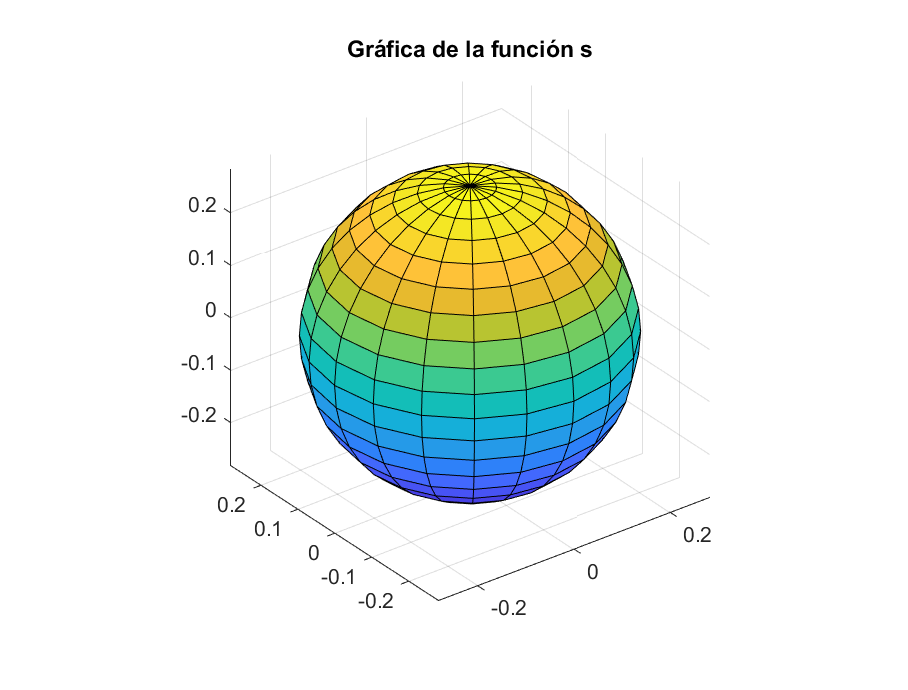
\includegraphics[scale=0.5]{Imagenes/Plot_Y00_Esfera.eps}
    %\caption{Gráfica del AER $Y_{0,0}$ en coordenadas esféricas polares.}
    %\label{fig:figura_plot_Y00}
\end{figure}
\end{frame}
\begin{frame}
\frametitle{Cuadrado del AER}
El cuadrado de esta función representa la contribución de la parte angular del orbital en la 
densidad de probabilidad.
\\
\bigskip
\pause
Pero como $[Y_{0,0}]^{2} = 0.076$ es también una constante, su gráfica es asimismo una esfera.
\end{frame}
\begin{frame}
\frametitle{Interpretaciónde la gráfica}
Lo que indica que \emph{la densidad de probabilidad de encontrar electrones es la misma independientemente de la dirección que se desee tomar (a partir del núcleo)}.
\end{frame}

% \subsection*{Las funciones \texorpdfstring{$p$}{p}.}

\begin{frame}
\frametitle{Las funciones $f$}
Nuevamente de la tabla de valores de los AER podemos reconocer que el factor de normalización:
\pause
\begin{align*}
A = (3/4 \pi)^{\frac{1}{2}} = 0.4886
\end{align*}
es el mismo para los tres armónicos esféricos tipo $p$. \pause Sin embargo, su dependencia angular resulta ser diferente, veremos que las tres funciones son equivalentes.
\end{frame}
\begin{frame}
\frametitle{El orbital $p_{z}$}
El orbital $p_{z}$ es la función:
\pause
\begin{align*}
p_{z} = 0.4886 \, \cos \theta
\end{align*}
\end{frame}
\begin{frame}
\frametitle{Gráfica de $p_{z}$}
Si graficamos la función coseno con el factor de normalización $A$, se tiene lo siguiente:
\pause
\begin{figure}[H]
    \centering
    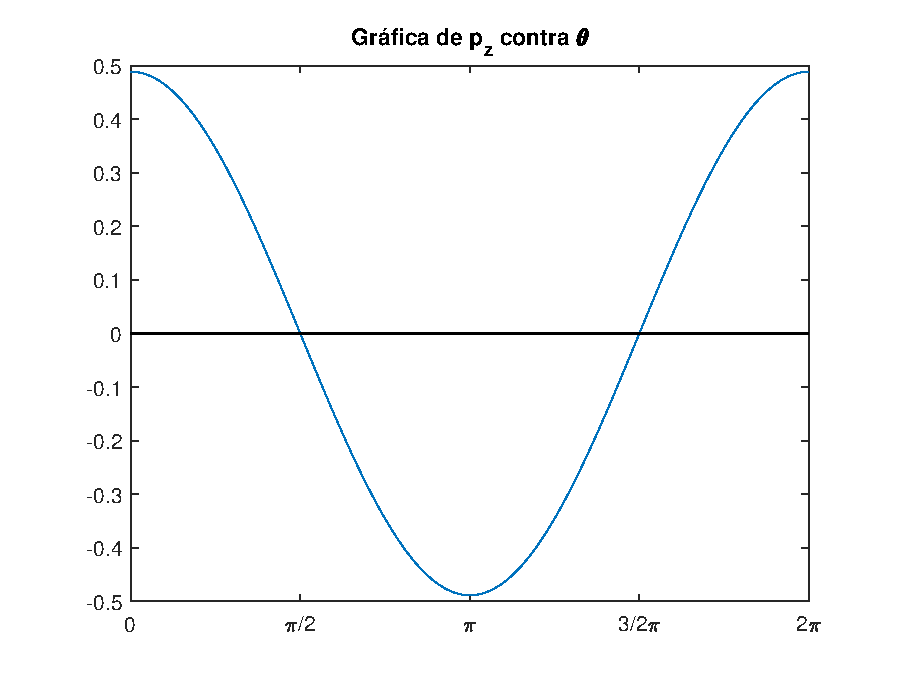
\includegraphics[scale=0.5]{Imagenes/Plot_AER_pz_theta.eps}
    %\caption{Gráfica de la función $p_{z}$ contra el ángulo $\theta$.}
    %\label{fig:plot_figura_pz_thetha}
\end{figure}
\end{frame}
\begin{frame}
\frametitle{Interpretando la gráfica}
Los valores de la función se representan como una distancia vertical, puede verse que la función toma valores negativos entre $\pi/2$ y $3 \pi/2$ y que su valor máximo ocurre en $\theta = \SI{0}{\degree}$.
\end{frame}
\begin{frame}
\frametitle{Gráfica en coordenadas esféricas}
Ahora graficamos $p_{z}$ en coordenadas esféricas polares sobre el plano $x-z$, incorporando la gráfica del cuadrado de $p_{z}$.
\\
\bigskip
\pause
El plano $x-z$ está compuesto por los dos hemiplanos con $\phi = \SI{0}{\degree}$ y $\phi = \SI{180}{\degree}$. \pause En cada uno de ellos hay que graficar midiendo a partir del eje $z$.
\end{frame}
\begin{frame}
\frametitle{Gráfica en coordenadas esféricas}
Al realizar esta tarea, tenemos la siguiente figura:
\pause
\begin{figure}[H]
    \centering
    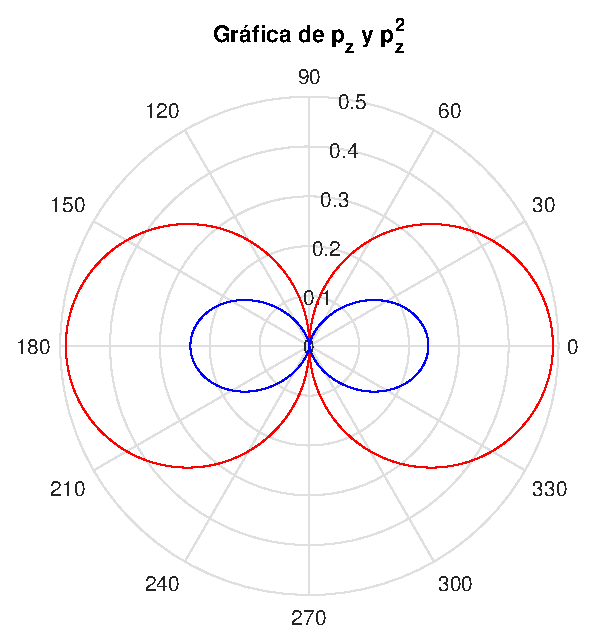
\includegraphics[scale=0.55]{Imagenes/Plot_AER_pz_theta_pz.eps}
    %\caption{Gráfica en coordenadas polares de $p_{z}$ y $p_{z}^{2}$ contra $\theta$.}
    %\label{fig:figura_plot_pz_pz2}
\end{figure}
\end{frame}
\begin{frame}
\frametitle{Estudiando la gráfica}
Notemos que por debajo del eje $x$ $(\theta > \SI{90}{\degree})$, la función $p_{z}$ es negativa, pero como lo que se grafica es su valor absoluto, se pierde esta información.
\end{frame}
\begin{frame}
\frametitle{Uso de signos}
Por ello, \emph{se acostumbra colocar un signo \enquote{más} en la región donde la función es positiva y un \enquote{menos} donde es negativa}.
\end{frame}
\begin{frame}
\frametitle{Valores donde se anula la función}
Para $\theta = \SI{90}{\degree}$ (ecuación del plano $x-y$), la función $p_{z}$ se anula, por lo que todo el plano $x-y$ es una superficie nodal.
\\
\bigskip
\pause
En este caso, para las funciones angulares las superficies nodales son planos.
\end{frame}
\begin{frame}
\frametitle{Estudiando la gráfica}
Mientras que para la gráfica $p_{z}$ resulta de dos círculos tangentes en el origen, su cuadrado tiene una forma oblonga.
\\
\bigskip
\pause
Así, la contribución angular a la densidad de probabilidad es mayor sobre las direcciones cercanas al eje $z$ y disminuye al alejarse de él, hasta anularse en el plano $x-y$.
\end{frame}
\begin{frame}
\frametitle{Simetría de la función}
La función $p_{z}$ es independiente del ángulo $\phi$, lo cual implica que es simétrica alrededor del eje $z$.
\\
\bigskip
\pause
La gráfica total de $p_{z}$ en coordenadas esféricas polares resulta ser un par de esferas tangentes en el origen colocadas sobre el eje $z$.
\end{frame}
\begin{frame}
\frametitle{Gráfica total de $p_{z}$}
\begin{figure}[H]
    \centering
    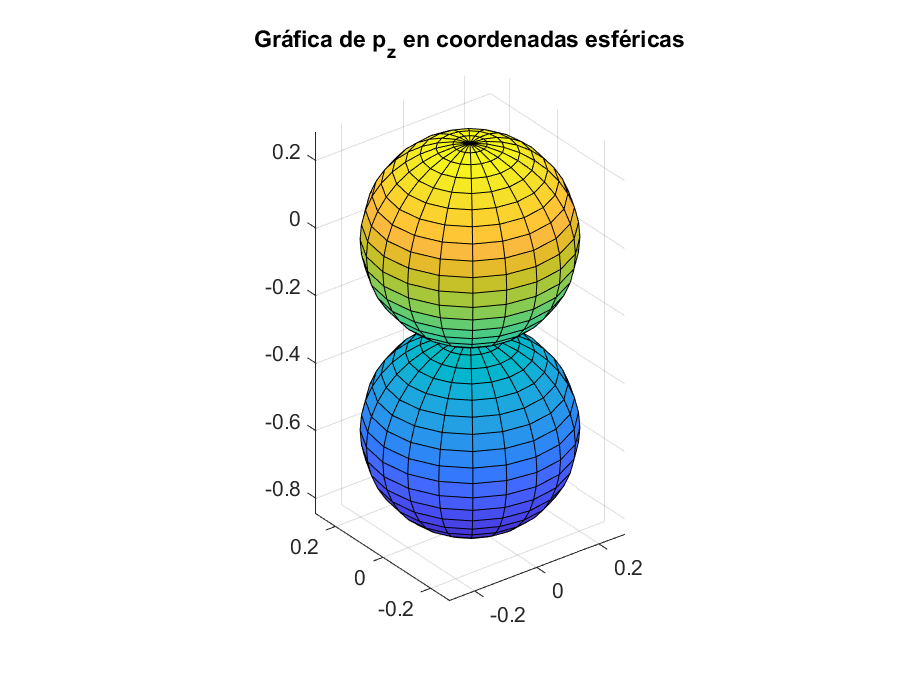
\includegraphics[scale=0.65]{Imagenes/Plot_AER_pz_theta_total3D.eps}
\end{figure}
\end{frame}
\begin{frame}
\frametitle{Las otras gráficas}
Las gráficas correspondientes a los orbitales $p_{x}$ y $p_{y}$ son equivalentes a la de $p_{z}$, con la diferencia de que las esferas están ahora colocadas sobre el eje $x$ y el eje $y$, respectivamente.
\end{frame}
\begin{frame}
\frametitle{Armónico esférico $Y_{1,0}$}
En la siguiente figura se presenta el armónico esférico $Y_{1,0} (\theta, \phi)$ que se recupera mediante Mathematica.
\\
\bigskip
\pause
El análisis que hemos presentado, nos da mucha más información que escribir un script y generar la figura.
\end{frame}
\begin{frame}
\frametitle{Gráfica del $Y_{0,0}$}
\begin{figure}[H]
    \centering
    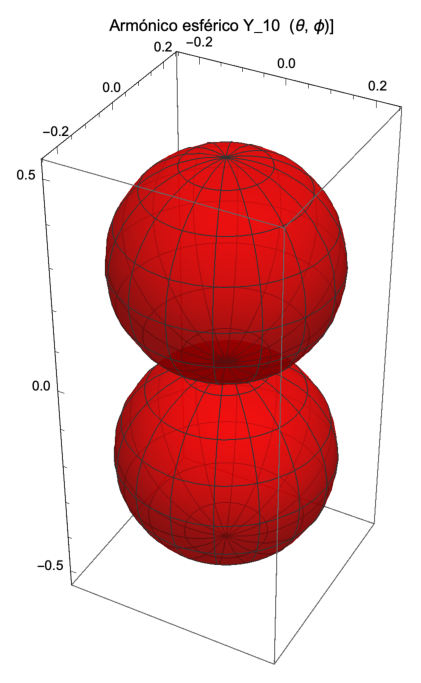
\includegraphics[scale=0.65]{Imagenes/Armonicos_Esfericos_10.eps}
\end{figure}
\end{frame}

\end{document}